\documentclass[11pt,a4paper]{article}
\usepackage[a4paper, margin=1.3in]{geometry}
\usepackage{mathtools}
\usepackage{graphicx}
\usepackage{fancyhdr}
\pagestyle{fancy}
\usepackage{lastpage}

\usepackage {tikz}
\usetikzlibrary {positioning}
%\usepackage {xcolor}
\definecolor {processblue}{cmyk}{0.96,0,0,0}

\fancyhf{}
\lhead{AI Planning}
\rhead{Exercise Sheet 4}
\lfoot{Axel Perschmann, Tarek Saier, 20.11.2014}
\rfoot{Page \thepage\ of \pageref{LastPage}}
\renewcommand{\headrulewidth}{0.3pt}
\renewcommand{\footrulewidth}{0.3pt}
\setlength\parindent{0pt}

\begin{document}
\begin{center}
\Huge{\textbf{AI Planning}}\\
\LARGE{\textbf{Exercise Sheet 4}}
\end{center}
\vspace{2cm}
\begin{tabular}{ll}
Date: & 20.11.2014\\
Students: & Axel Perschmann, Tarek Saier
\end{tabular}

\section*{Exercise 4.1}
For easy readability let the tiles be referred to as $b_1$, $b_2$, $w_1$ and $w_2$ and the empty cell be referred to as $e$. Furthermore, let the actions move and jump be denoted as $m_c(t)$ and $j_c(t)$ respectively where $c$ is the destination cell$\in \{1,2,3,4,5\}$ and $t$ is the tile that is being relocated.\\
As an example, the initial state is:\\
$b_1,b_2,w_1,w_2,e$\\
If we then apply $j_5(b_2)$ we reach:\\
$b_1,e,w_1,w_2,b_2$\\
\\
\textbf{(a)} Let $\lceil o\rceil$ denote the state $s$ reached by applying the operation $o\in \{m_c(t),j_c(t)\}$.\\
$f(\lceil m_5(w_2)\rceil)=1+4=5$\\
$f(\lceil j_5(w_1)\rceil)=1+4=5$\\
$f(\lceil j_5(b_2)\rceil)=2+2=4$\\
Apply $j_5(b_2)$ which results in $s_1$:\\
$b_1,e,w_1,w_2,b_2$\\
$f(\lceil m_2(b_1)\rceil)=3+2=5$\\
$f(\lceil m_2(w_1)\rceil)=3+2=5$\\
$f(\lceil j_2(w_2)\rceil)=3+2=5$\\
$\lceil j_2(b_2)\rceil=I\in closed$\\
Apply $m_2(b_1)$ which results in $s_2$:\\
$e,b_1,w_1,w_2,b_2$\\
Apply $m_2(w_1)$ which results in $s_3$:\\
$b_1,w_1,e,w_2,b_2$\\
Apply $j_2(w_2)$ which results in $s_4$:\\
$b_1,w_2,w_1,e,b_2$\\
Expanding on $s_2$:\\
$\lceil m_1(b_1)\rceil=s_1\in closed$\\
$f(\lceil j_1(w_1)\rceil)=4+1=5$\\
$f(\lceil j_1(w_2)\rceil)=5+1=6$\\
Expanding on $s_3$:\\
$f(\lceil j_3(b_1)\rceil)=4+1=5$\\
$f(\lceil m_3(w_1)\rceil)=4+2=6$\\
$f(\lceil m_3(w_2)\rceil)=4+2=6$\\
$f(\lceil j_3(b_2)\rceil)=4+3=7$\\
\\
Expanding on $s_4$:\\
$f(\lceil j_4(b_1)\rceil)=5+0=5$\\
\\
Since $h$ is goal aware and the minimum cost of an operator is 1 we're done at this point. There may be other solutions but none with a cost of less than 5. The resulting plan is: $j_5(b_2),j_2(w_2),j_4(b_1)$ with a total cost of 5 and a final state:\\
$e,w_2,w_1,b_1,b_2$\\

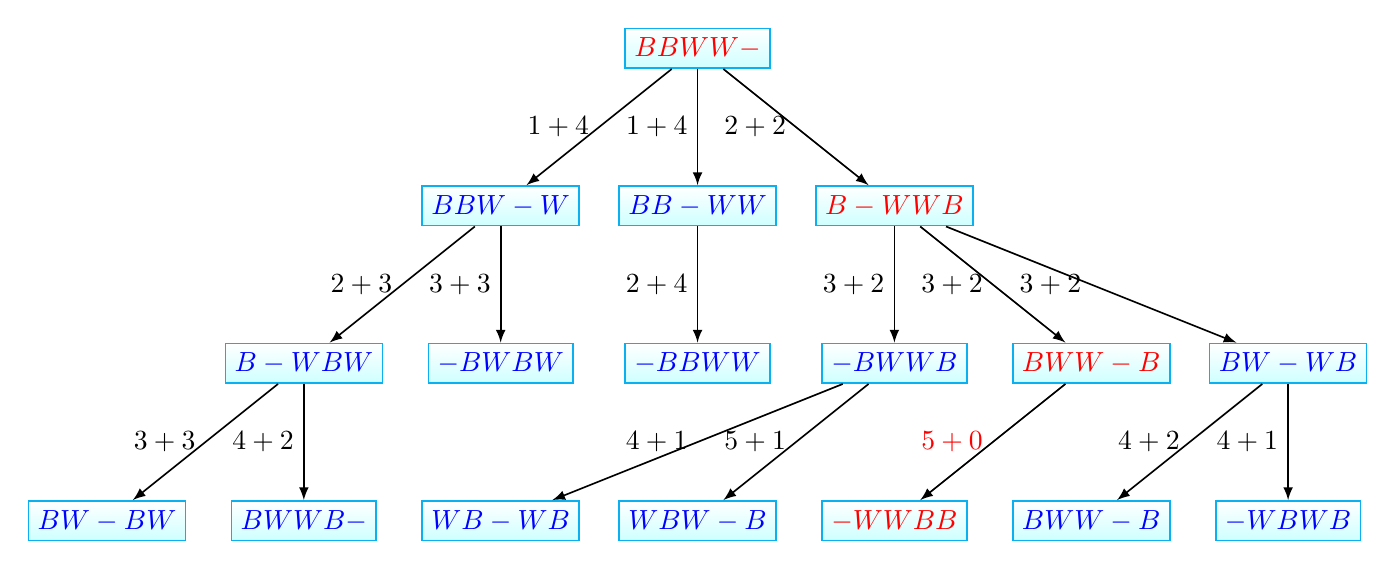
\begin{tikzpicture}[-latex ,auto ,node distance =2 cm and 2.5cm ,on grid ,
semithick ,
state/.style ={top color =white , bottom color = processblue!20 ,
draw,processblue , text=blue },
goalstate/.style ={top color =white , bottom color = processblue!20 ,
draw,processblue , text=red }]
\node[goalstate] (A) {$BBWW-$};
\node[state] (B1) [below left=of A] {$BBW-W$};
\node[state] (B2) [right =of B1] {$BB-WW$};
\node[goalstate] (B3) [right =of B2] {$B-WWB$};
\path (A) edge node[left] {$1+4$} (B1);
\path (A) edge node[left] {$1+4$} (B2);
\path (A) edge node[left] {$2+2$} (B3);
\node[state] (C2) [below =of B1] {$-BWBW$};
\node[state] (C1) [left =of C2] {$B-WBW$};
\path (B1) edge node[left] {$2+3$} (C1);
\path (B1) edge node[left] {$3+3$} (C2);
\node[state] (C3) [below =of B2] {$-BBWW$};
\path (B2) edge node[left] {$2+4$} (C3);
\node[state] (C4) [below =of B3] {$-BWWB$};
\node[goalstate] (C5) [right=of C4] {$BWW-B$};
\node[state] (C6) [right=of C5] {$BW-WB$};
\path (B3) edge node[left] {$3+2$} (C4);
\path (B3) edge node[left] {$3+2$} (C5);
\path (B3) edge node[left] {$3+2$} (C6);
\node[goalstate] (D1) [below left =of C5] {$-WWBB$};
\path (C5) edge node[left] {\textcolor{red}{$5+0$}} (D1);

\node[state] (E1) [below left =of C1] {$BW-BW$};
\node[state] (E2) [right =of E1] {$BWWB-$};
\path (C1) edge node[left] {$3+3$} (E1);
\path (C1) edge node[left] {$4+2$} (E2);

\node[state] (F2) [below left =of C4] {$WBW-B$};
\node[state] (F1) [left =of F2] {$WB-WB$};
\path (C4) edge node[left] {$4+1$} (F1);
\path (C4) edge node[left] {$5+1$} (F2);

\node[state] (G1) [below left =of C6] {$BWW-B$};
\node[state] (G2) [right =of G1] {$-WBWB$};
\path (C6) edge node[left] {$4+2$} (G1);
\path (C6) edge node[left] {$4+1$} (G2);
\end{tikzpicture}
\vspace{10 mm}

\textbf{(b)} Suppose we loosened the rules of our puzzle in the following way: there are infinitely many empty cells left of the leftmost $b_i$ and right of the rightmost $w_j$. Furthermore jumps over more than 2 tiles are allowed while the calculation of cost follows the original rule but never exceeds 2.\\
In this relaxed setting the puzzle can always be solved at a cost of\\
\begin{equation*}
h_r^*(s) = \sum_{i=1}^{\text{number of black tiles}} b_i\times \text{number of white tiles right of }b_i
\end{equation*}
Since this is a less restrictive setting $h_r^*(s)\leq h^*(s)$. Furthermore $h_r^*(s)$ is a more general variant of $h(s)$. In other words, for the specific case $I$ we can say $h_r^*(s)=h(s)$ and therefore $h(s)\leq h^*(s)$.

\section*{Exercise 4.2}
Start conditions: $\sigma_0 =\{H_x=1, H_y=2, G_x=4, G_y=4\}$, $h(\sigma_0)=5$\\
Possible actions:\\$northH, south_H, east_H, west_H, north_G, south_G, east_G, west_G$\\

\begin{enumerate}
\item
$improve(\sigma_0)$ iterates over possible successor states of $\sigma_0$, until $h(\sigma_1) < h(\sigma_0)$\\
\begin{tabular}{l r}
$\sigma_1 = \langle{}\sigma_0, north_H, \{H_x=1, H_y=3, G_x=4, G_y=4\}\rangle$ & $h(\sigma_1)=4$
\end{tabular}\\
$h(\sigma_1) < h(\sigma_0)$ is causing the end of $improve(\sigma_0)$

\item
$\sigma_1$ is not a goal-state yet, thus improve($\sigma_1$) is called.\\
\begin{tabular}{l r}
$\sigma_{2} = \langle{}\sigma_1, east_H, \{H_x=2, H_y=3, G_x=4, G_y=4\}\rangle$ & $h(\sigma_{2})=3$
\end{tabular}\\
$h(\sigma_2) < h(\sigma_1)$ is causing the end of $improve(\sigma_1)$

\item
 $\sigma_2$ is not a goal-state yet, thus improve($\sigma_2$) is called.\\
\begin{tabular}{l r}
$\sigma_{3} = \langle{}\sigma_{2}, east_H, \{H_x=3, H_y=3, G_x=4, G_y=4\}\rangle$ & $h(\sigma_{3})=2$
\end{tabular}\\
$h(\sigma_3) < h(\sigma_2)$ is causing the end of $improve(\sigma_2)$

\item
 $\sigma_3$ is not a goal-state yet, thus improve($\sigma_3$) is called.\\
\begin{tabular}{l r}
$\sigma_{4} = \langle{}\sigma_{3}, south_H, \{H_x=3, H_y=2, G_x=4, G_y=4\}\rangle$ & $h(\sigma_{4})=3$\\
$\sigma_{5} = \langle{}\sigma_{3}, north_G, \{H_x=3, H_y=3, G_x=4, G_y=5\}\rangle$ & $h(\sigma_{5})=3$\\
$\sigma_{6} = \langle{}\sigma_{3}, east_G, \{H_x=3, H_y=3, G_x=5, G_y=4\}\rangle$ & $h(\sigma_{6})=3$
\end{tabular}

\item
No improvement happened, $improve(\sigma_3)$ still running.\\
Enforced hill-climbing algorithm will collect all successor states of $\sigma_4$, $\sigma_5$ and $\sigma_6$ for an improvement.\\
To make sure this solution sheet will not explode in size, we'll only have a look on the most suitable steps, in this case $\sigma_6$\\
\begin{tabular}{l r}
$\sigma_{7} = \langle{}\sigma_{6}, south_H, \{H_x=3, H_y=2, G_x=5, G_y=4\}\rangle$ & $h(\sigma_{7})=4$\\
$\sigma_{8} = \langle{}\sigma_{6}, north_G, \{H_x=3, H_y=3, G_x=5, G_y=5\}\rangle$ & $h(\sigma_{8})=4$\\
$\sigma_{9} = \langle{}\sigma_{6}, south_G, \{H_x=3, H_y=3, G_x=5, G_y=3\}\rangle$ & $h(\sigma_{9})=2$
\end{tabular}\\
$h(\sigma_9) < h(\sigma_6)$ is causing the end of $improve(\sigma_6)$

\item
 $\sigma_9$ is not a goal-state yet, thus improve($\sigma_9$) is called.\\
 \begin{tabular}{l r}
 $\sigma_{10} = \langle{}\sigma_{9}, south_G, \{H_x=3, H_y=3, G_x=5, G_y=2\}\rangle$ & $h(\sigma_{10})=3$\\
 \end{tabular}
 
 \item
No improvement happened, $improve(\sigma_9)$ still running.\\
 \begin{tabular}{l r}
 $\sigma_{11} = \langle{}\sigma_{10}, west_G, \{H_x=3, H_y=3, G_x=4, G_y=2\}\rangle$ & $h(\sigma_{11})=2$\\
  \end{tabular}
 
  \item
No improvement happened, $improve(\sigma_9)$ still running.\\
 \begin{tabular}{l r}
 $\sigma_{12} = \langle{}\sigma_{11}, south_G, \{H_x=3, H_y=3, G_x=4, G_y=1\}\rangle$ & $h(\sigma_{12})=3$\\
 $\sigma_{13} = \langle{}\sigma_{11}, west_G, \{H_x=3, H_y=3, G_x=3, G_y=2\}\rangle$ & $h(\sigma_{13})=1$\\
 \end{tabular}\\
$h(\sigma_{13}) < h(\sigma_9)$ is causing the end of $improve(\sigma_9)$
 
\item
 $\sigma_{13}$ is not a goal-state yet, thus improve($\sigma_{13}$) is called.\\ 
  \begin{tabular}{l r}
 $\sigma_{14} = \langle{}\sigma_{13}, north_G, \{H_x=3, H_y=3, G_x=3, G_y=3\}\rangle$ & $h(\sigma_{14})=0$
  \end{tabular}\\
$h(\sigma_{14}) < h(\sigma_{13})$ is causing the end of $improve(\sigma_{13})$

\item
 $\sigma_{14}$ is a goal-state, thus $extract\_solution(\sigma_{14})$ is called.\\
\end{enumerate}

The solution found by the enforced hill-climbing algorithm:\\
${north_H, east_H, east_H, east_G, south_G, south_G, west_G, west_G, north_G}$

cost/number of steps: 9




\end{document}
